\section{Implementierung}

Die Implementierung gestalltete sich \"uberwiegend in der main.c. Da diese mit am schlechtesten auskommentiert war, war eine Rekapitulaion des bereits vorhandenen Quellcodes sehr schwierig. Wir entschlossen uns daher die main.c schrittweise neu herzuleiten und die Verwendung der einzelnen Headerdateien zu verstehen. Die ersten GUIs die somit entstanden waren einfache Konstrukte aus Linien und Text. Im n\"achsten Schritt implementierten wir die ersten Buttons und die dazugeh\"origen Funktionen. Aufbauend darauf enstand ein simpler Taschenrechner f\"ur dessen Eingabe ein 3x4 Pinpad und jeweils ein Button f\"ur die jeweilige Grundrechenart. Wir kamen danach zu dem Punkt an dem wir uns ein Konzept f\"ur die eigentliche Nutzeroberfl\"ache \"uberlegen mussten. Dabei entschieden wir uns f\"ur die Men\"uf\"uhrung welche bereits in der orgninalen main.c implementiert war, da diese durch die Men\"uauswahl auf der rechten Displayseite eine intuitive Bedienung erm\"oglichte. Die Men\"upunkte erm\"oglichen dem Nutzer Zugriff auf die Enrollement-, Verifikations- u. Konfigurationsfunktionen zu nehmen. Nach der Initialisierung wird auf dem Display eine Willkommensanzeige dargestellt. (Abbildung \ref{welcScreen}) Beim Enrollement und der Verifikation werden jeweils 8 Buttons angezeigt welche f\"ur die Auswahl des aktuellen Nutzers zust\"adnig sind. Die Buttons wurden einem Frame in der Anordung 4x2 zugeordnet, damit mussten wir die Buttons nicht einzeln zeichnen lassen sondern konnten durch ein einmaliges zeichnen des Frames alle Buttons darstellen. (Abbildung \ref{Pic2}) Um den Quellcode weiterhin zu verk\"urzen nutzten wir den Frame mit den Buttons wie bereits erw\"ahnt sowohl f\"ur den Enrollementprozess sowie f\"ur die Verifikation. Das hei{\ss}t bei einem Klickevent wird die Abfrage gestellt welche Men\"upunkt aktiviert ist und erst danach erfolgt der Aufruf der Funktion. Diese Funktion ist bisweilen aber nur f\"ur User1 implementiert. Um die Tresholdeinstellung aus dem Konfigurationsmen\"u in die Verifikation mit einflie{\ss}en zu lassen haben wir die Funktion daf\"ur geringf\"ugig modifiziert. Wir haben einen zus\"atzlichen \"Ubergabeparameter und eine Abfrage ob die Hammingdistanz den gesetzten Treshold \"uberschritten hat hinzugef\"ugt. Ausserdem erfolgt in der Funktion noch die Ausgabe ob die Verifikation erfolgreich war oder eben nicht.(Abbildung \ref{Pic3}) Das zweite Frame ist demzufolge f\"ur das Konfigurationsmen\"u geschaffen. Dort besteht die M\"oglichkeit den Treshold f\"ur eine g\"ultige bzw. ung\"ultige Verifikation auf die Werte 5, 10, 15 und 20 zu setzten (Abbildung \ref{TreshScreen}). Sollte hier keine weitere Einstellung des Nutzers erfolgen wird die Verifikation mit einem Treshold von 10 durchgef\"uhrt. \footnote{\label{foot:1} Quellcode: \ref{quellcode}}

 \begin{figure}
  \centering
  \subfloat[]{\label{welcScreen}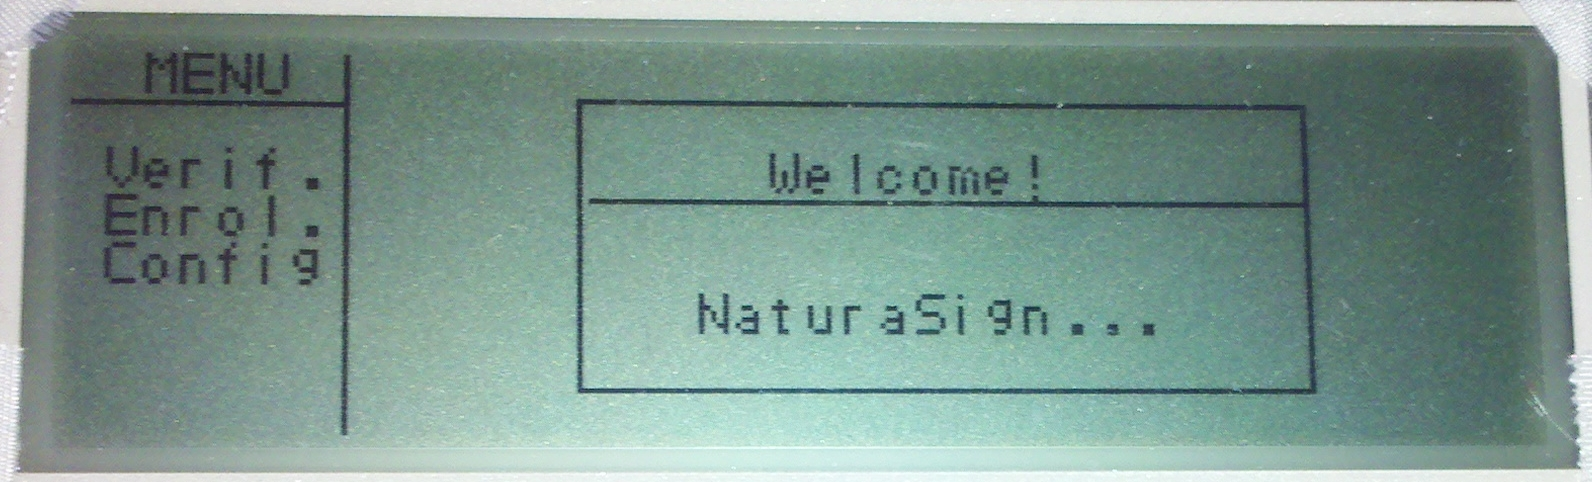
\includegraphics[width=0.5\textwidth]{img/welcScreen.jpg}}
  \subfloat[]{\label{TreshScreen}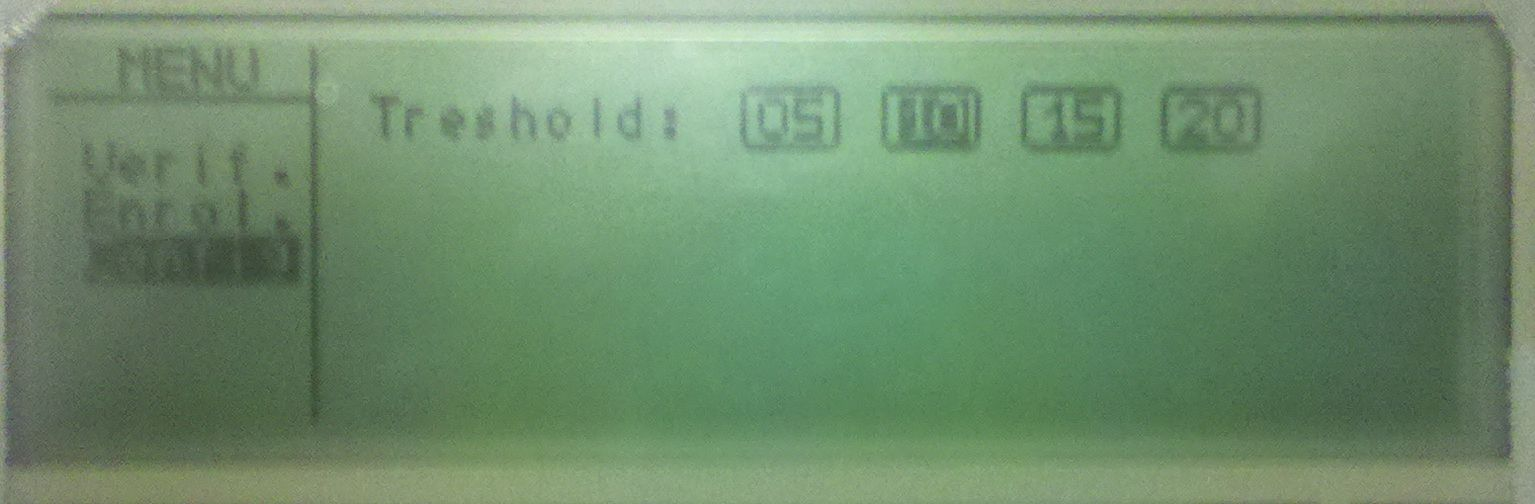
\includegraphics[width=0.46\textwidth]{img/TreshScreen.jpg}}
  \caption{Willkommensanzeige und Konfigurationsmen\"u}
  \label{Pic1}
\end{figure}

 \begin{figure}
  \centering
  \subfloat[]{\label{veriScreen}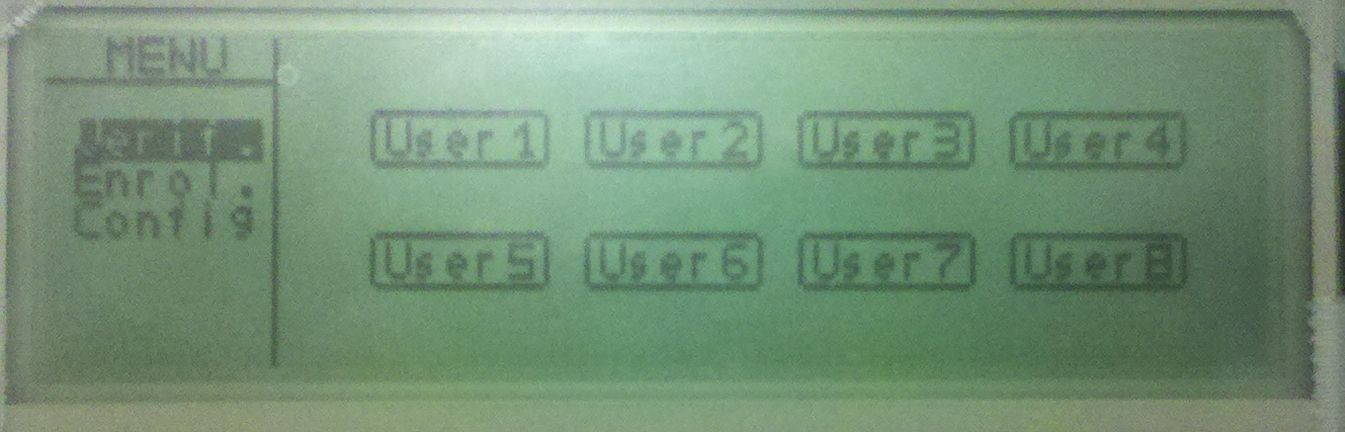
\includegraphics[width=0.5\textwidth]{img/veriScreen.jpg}}
  \subfloat[]{\label{enrolScreen}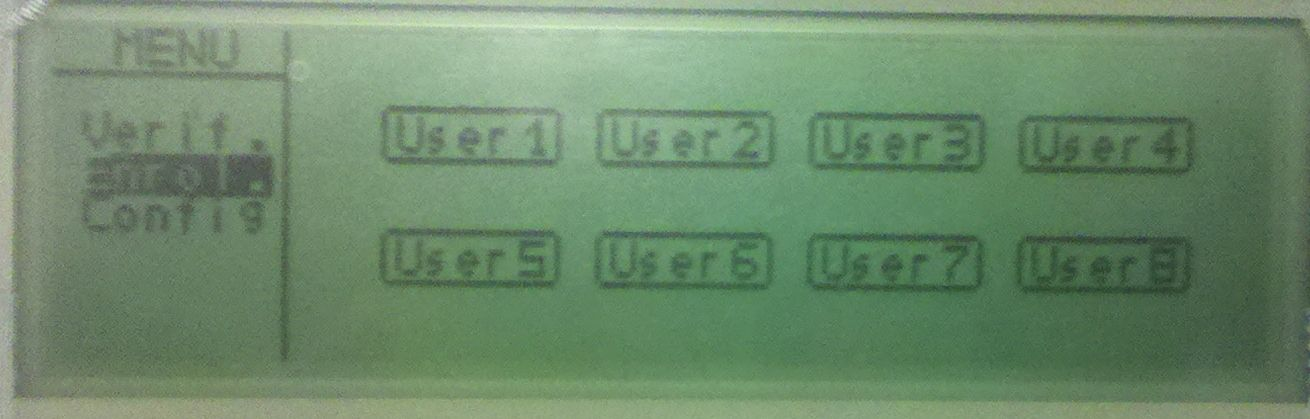
\includegraphics[width=0.50\textwidth]{img/enrolScreen.jpg}}
  \caption{Nutzerauswahl beim Enrollment und der Verifikation}
  \label{Pic2}
\end{figure}

 \begin{figure}
  \centering
  \subfloat[]{\label{failScreen}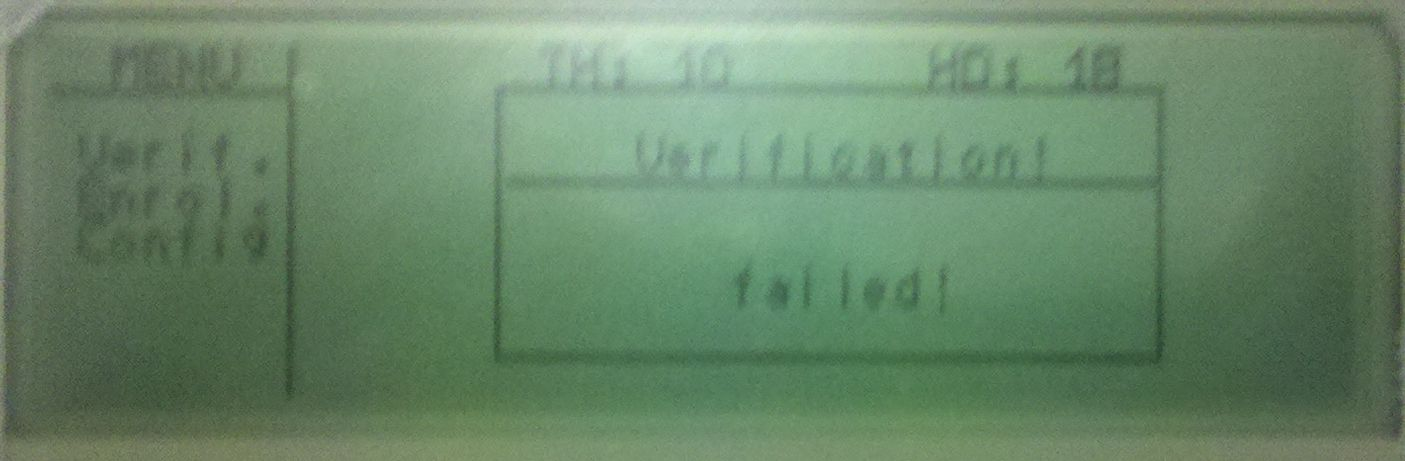
\includegraphics[width=0.48\textwidth]{img/failScreen.jpg}}
  \subfloat[]{\label{succesScreen}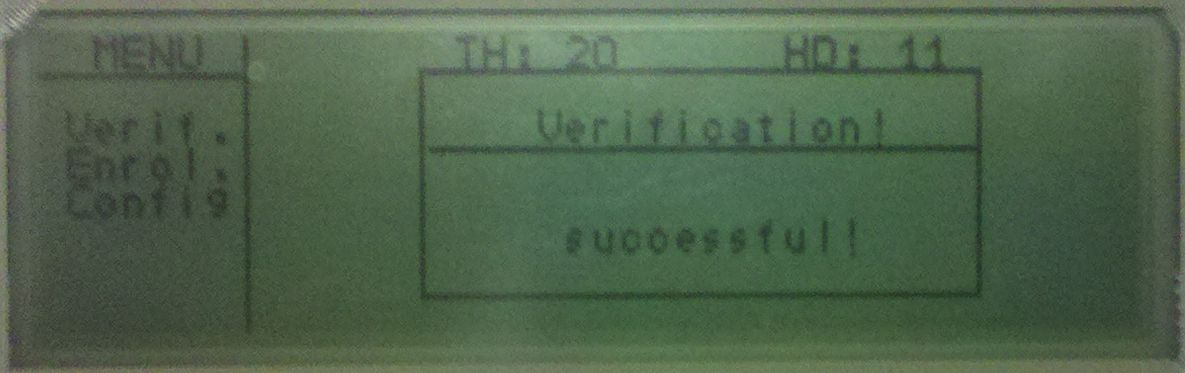
\includegraphics[width=0.50\textwidth]{img/succesScreen.jpg}}
  \caption{Ergebnisse der Verifikation}
  \label{Pic3}
\end{figure}

		
	\begin{figure}
  	\centering
  	\fbox{
    	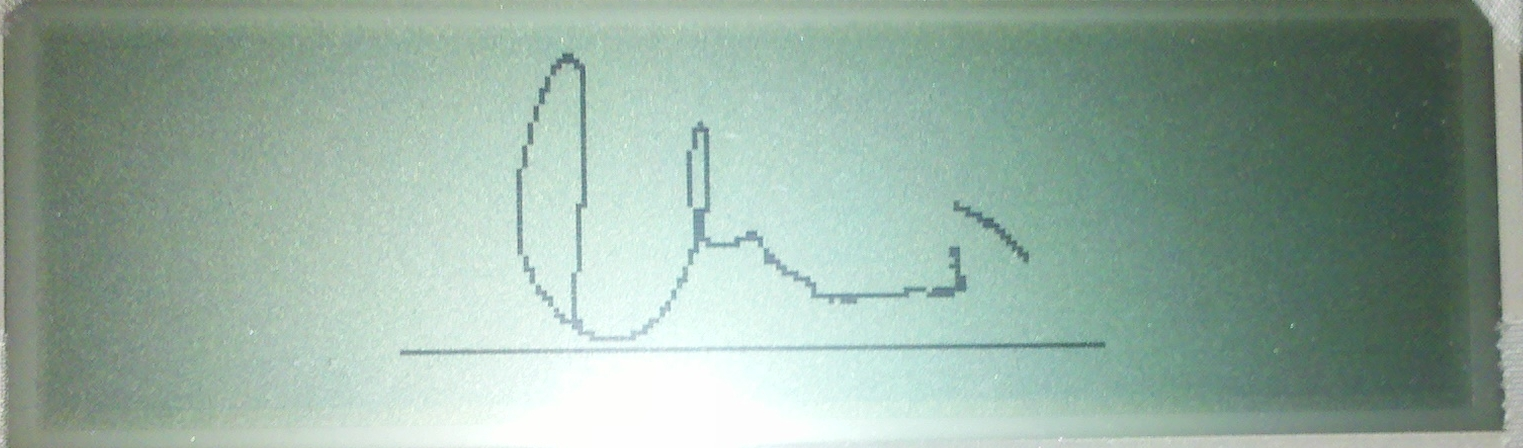
\includegraphics[scale=0.70]{img/graphScreen.jpg}
  	}
  	\caption{Unterschrift}
  	\label{graphScreen}
	\end{figure}
	
		
	